This section describes the model built to represent the world in which the \verb|eMALL| system works.

\section{Alloy Code}
\label{sec:alloy}%
\begin{lstlisting}[language=alloy,label={lst:alloy_code}]
open util/ordering[DateTime]

sig Appointment {
	startDate : DateTime,
	endDate : DateTime,
	chargingPoint : ChargingPoint
} {this in Calendar.appointments}

sig Battery {} {this in ChargingStation.batteries}

sig Calendar {appointments : disj set Appointment} {this in EVD.calendar}

sig ChargingPoint {
	eV : disj lone EV,
	plugs : some Plug
} {
	EV.plug in plugs and
	this in ChargingStation.chargingPoints
}

sig ChargingStation {
	chargingPoints : disj some ChargingPoint,
	batteries : disj set Battery,
	wayOfCharging : disj Battery + DSO
} {this in CPO.chargingStations}

sig CPO {
	chargingStations : disj some ChargingStation,
	dso : DSO
}

sig DateTime {} {this in Appointment.startDate + Appointment.endDate}

sig DSO {} {this in CPO.dso}

sig Email {} {this in EVD.email}

sig EV {plug : Plug} {this in UnregisteredEVD.eVs + EVD.eVs}

sig EVD {
	calendar : disj Calendar,
	email : disj Email,
	eVs : disj some EV,
	password : disj Password
}

sig Password {} {this in EVD.password}

abstract sig Plug {}
one sig CCS extends Plug {}
one sig ChaDeMo extends Plug {}
one sig Type1 extends Plug {}
one sig Type2 extends Plug {}

sig UnregisteredEVD {eVs : disj some EV}

/************************************************************************************/
/************************************************************************************/

///* An EVD cannot charge his EVs simultaneously, we assume each account is associated to only one driver
fact evdsCanChargeOnlyOneEvPerTime {
	all evd : EVD, disj ev1, ev2 : EV |
		ev1 + ev2 in evd.eVs and
		ev1 in ChargingPoint.eV implies
			ev2 not in ChargingPoint.eV
}
///* An appointment must start before ending
fact appointmentsAreCorrect {
	all a : Appointment |
		lt [a.startDate, a.endDate]
}
///* A booking process must not be overlapped to another booking process in the same calendar and in the same charging point
fact noOverlappedAppointmentsInChargingPointSchedules {
	no disj a1, a2 : Appointment |
		a1.chargingPoint in a2.chargingPoint and
		gte [a1.startDate, a2.startDate] and
		lte [a1.startDate, a2.endDate]
	no c : Calendar, disj a1, a2 : c.appointments |
		gte [a1.startDate, a2.startDate] and
		lte [a1.startDate, a2.endDate]
}
///* EVs of EVDs are not shared with unregistered EVDs
fact evsOfEvdsAreNotSharedWithUnregisteredEvds {
	all evd : EVD, uevd : UnregisteredEVD |
		#(evd.eVs & uevd.eVs) = 0
}
///* EVs of unregistered EVDs must not be connected to charging points
fact evsOfUnregisteredEvdsMustNotBeConnectedToChargingPoints {
	all cp : ChargingPoint, uevd : UnregisteredEVD |
		#(cp.eV & uevd.eVs) = 0
}
///* Charging stations charge vehicles through their batteries and DSOs
fact chargingStationsUseTheirBatteries {
	all cs : ChargingStation, cpo : CPO |
		cs in cpo.chargingStations and
		cs.wayOfCharging in cs.batteries + cpo.dso
}

/************************************************************************************/
/************************************************************************************/

///* EVs are connected to compatible charging points
assert evsAreConnectedToCompatibleChargingPoints {
	no cp : ChargingPoint |
		cp.eV.plug not in cp.plugs
}
///* No overlapped appointments in charging point schedules
assert noOverlappedAppointmentsInChargingPointSchedules {
	no disj a1, a2 : Appointment |
		a1.chargingPoint in a2.chargingPoint and
			lte [a1.startDate, a2.startDate] and
			lte [a1.endDate, a2.startDate]
}

/************************************************************************************/
/************************************************************************************/

///* Add new appointment to the calendar for an EVD
pred addNewAppointmentToCalendarForEvd [evd : EVD, a' : Appointment] {
	evd.calendar.appointments = evd.calendar.appointments + a'
}
///* Add new charging point to a charging station
pred addNewChargingPointToChargingStation [cs : ChargingStation, cp' : ChargingPoint] {
	cs.chargingPoints = cs.chargingPoints + cp'
}
///* Add new charging station to a CPO
pred addNewChargingStationToCpo [cpo : CPO, cs' : ChargingStation] {
	cpo.chargingStations = cpo.chargingStations + cs'
}
///* Add new EV to an EVD
pred addNewEvToEvd [evd : EVD, ev' : EV] {
	evd.eVs = evd.eVs + ev'
}
///* Add new plug in a charging point
pred addNewPlugToChargingPoint [cp : ChargingPoint, p' : Plug] {
	cp.plugs = cp.plugs + p'
}
///* Remove appointment from the calendar of an EVD
pred removeAppointmentFromCalendarOfEvd [evd : EVD, a : Appointment] {
	evd.calendar.appointments = evd.calendar.appointments - a
}
///* Remove a charging point from a charging station
pred removeChargingPointFromChargingStation [cs : ChargingStation, cp : ChargingPoint] {
	cs.chargingPoints = cs.chargingPoints - cp
}
///* Remove a charging station from a CPO
pred removeChargingStationFromCpo [cpo : CPO, cs : ChargingStation] {
	cpo.chargingStations = cpo.chargingStations - cs
}
///* Remove EV from an EVD
pred removeEvFromEvd [evd : EVD, ev : EV] {
	evd.eVs = evd.eVs - ev
}
///* Remove plug from a charging point
pred removePlugFromChargingPoint [cp : ChargingPoint, p : Plug] {
	cp.plugs = cp.plugs - p
}
///* Update email in an EVD
pred updateEmailInEvd [evd : EVD, e' : Email] {
	evd.email = e'
}
///* Create a simple world
pred simpleWorld {
	#ChargingStation = 1
	#ChargingPoint = 3
	#EVD = 2
	#Appointment = 2
}
///* Create a world where there are many appointments
pred worldWithManyAppointments {
	#ChargingStation = 1
	#ChargingPoint = 4
	#EVD = 2
	#Appointment = 6
}

/************************************************************************************/
/************************************************************************************/

run addNewAppointmentToCalendarForEvd

run addNewChargingPointToChargingStation

run addNewChargingStationToCpo

run addNewEvToEvd

run addNewPlugToChargingPoint

run removeAppointmentFromCalendarOfEvd

run removeChargingPointFromChargingStation

run removeChargingStationFromCpo

run removeEvFromEvd

run removePlugFromChargingPoint

run updateEmailInEvd

run simpleWorld

run worldWithManyAppointments for 10

check evsAreConnectedToCompatibleChargingPoints

check noOverlappedAppointmentsInChargingPointSchedules
\end{lstlisting}

\section{Simulations}
\label{sec: sim}%
In this section we show to simulations of the built model.
The first one is a simple world, with few instances, useful to understand the basis of the relations between entities.
The second world is more complex due to the representation of a higher number of instances of stations, EVDs and appointments.

\begin{sidewaysfigure}
	\begin{figure} [H]
		\begin{center}
			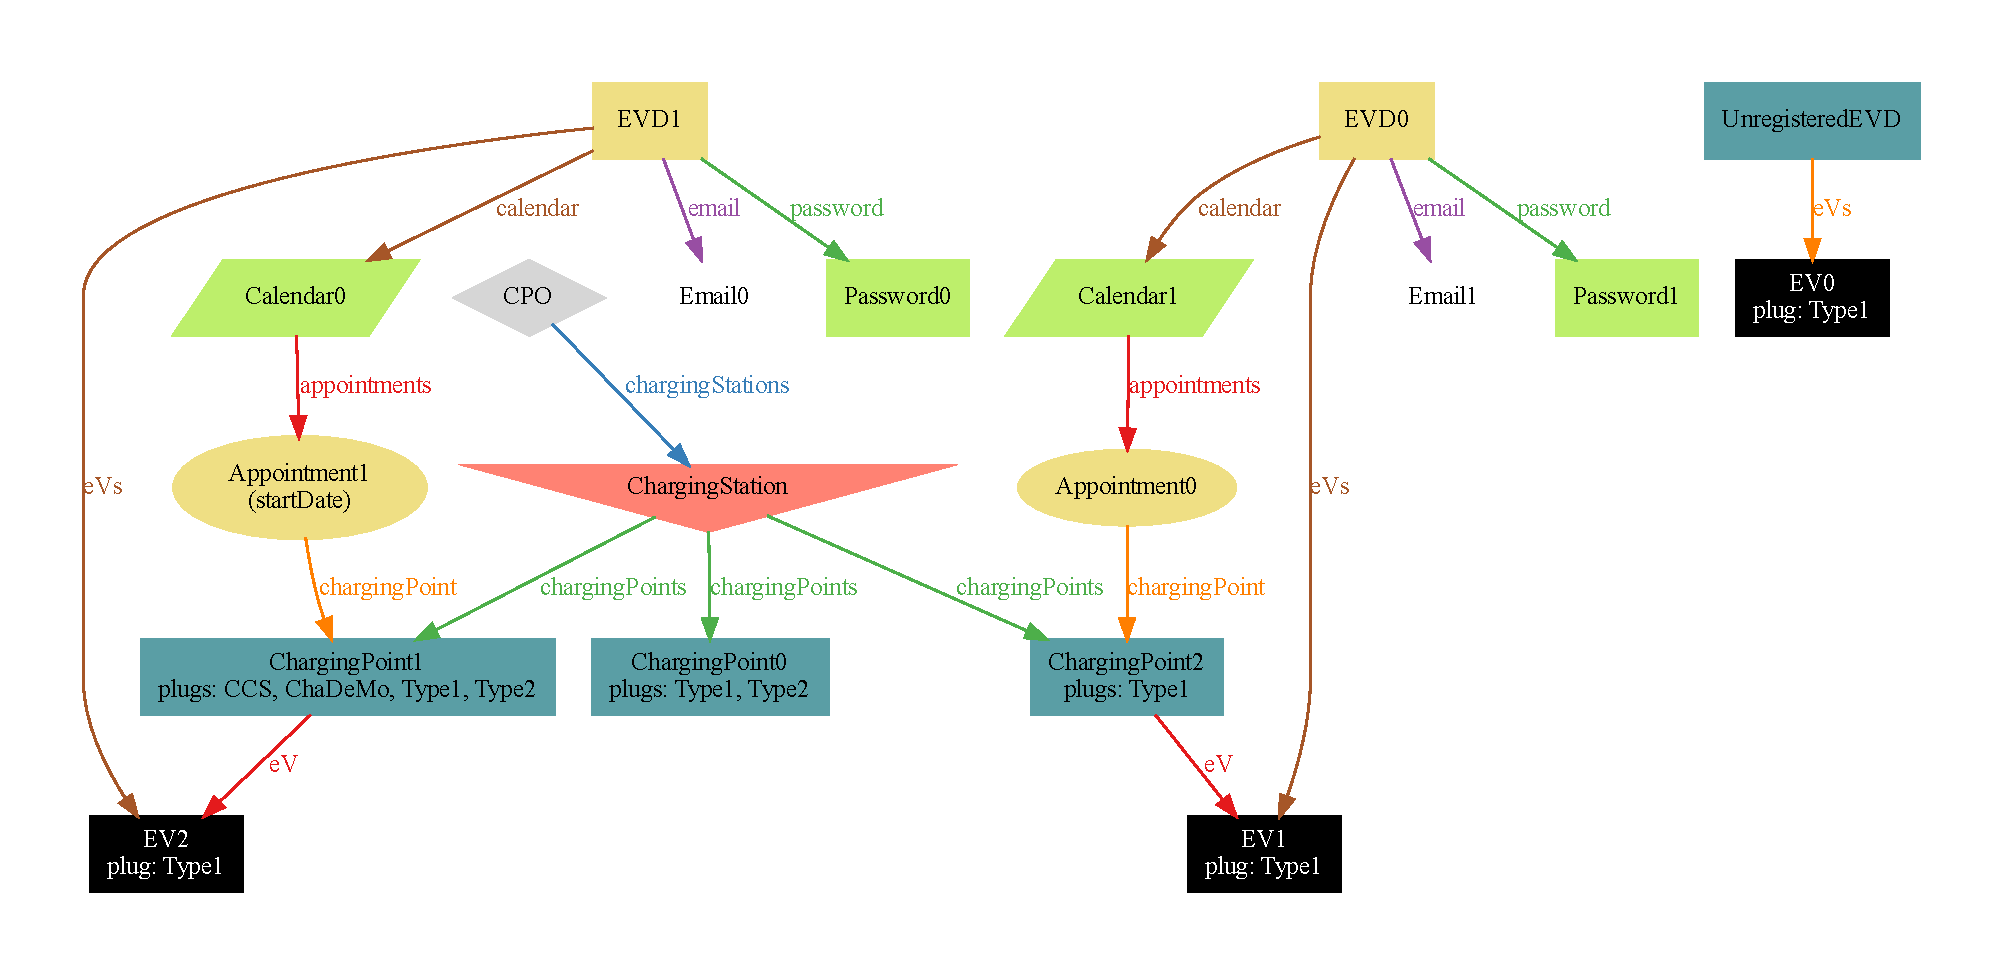
\includegraphics[width=1\linewidth]{graphs/simpleWorld}
			\caption{Simple world Alloy.}
			\label{fig: simple_world_alloy}
		\end{center}
	\end{figure}
\end{sidewaysfigure}

\begin{sidewaysfigure}
	\begin{figure} [H]
		\begin{center}
			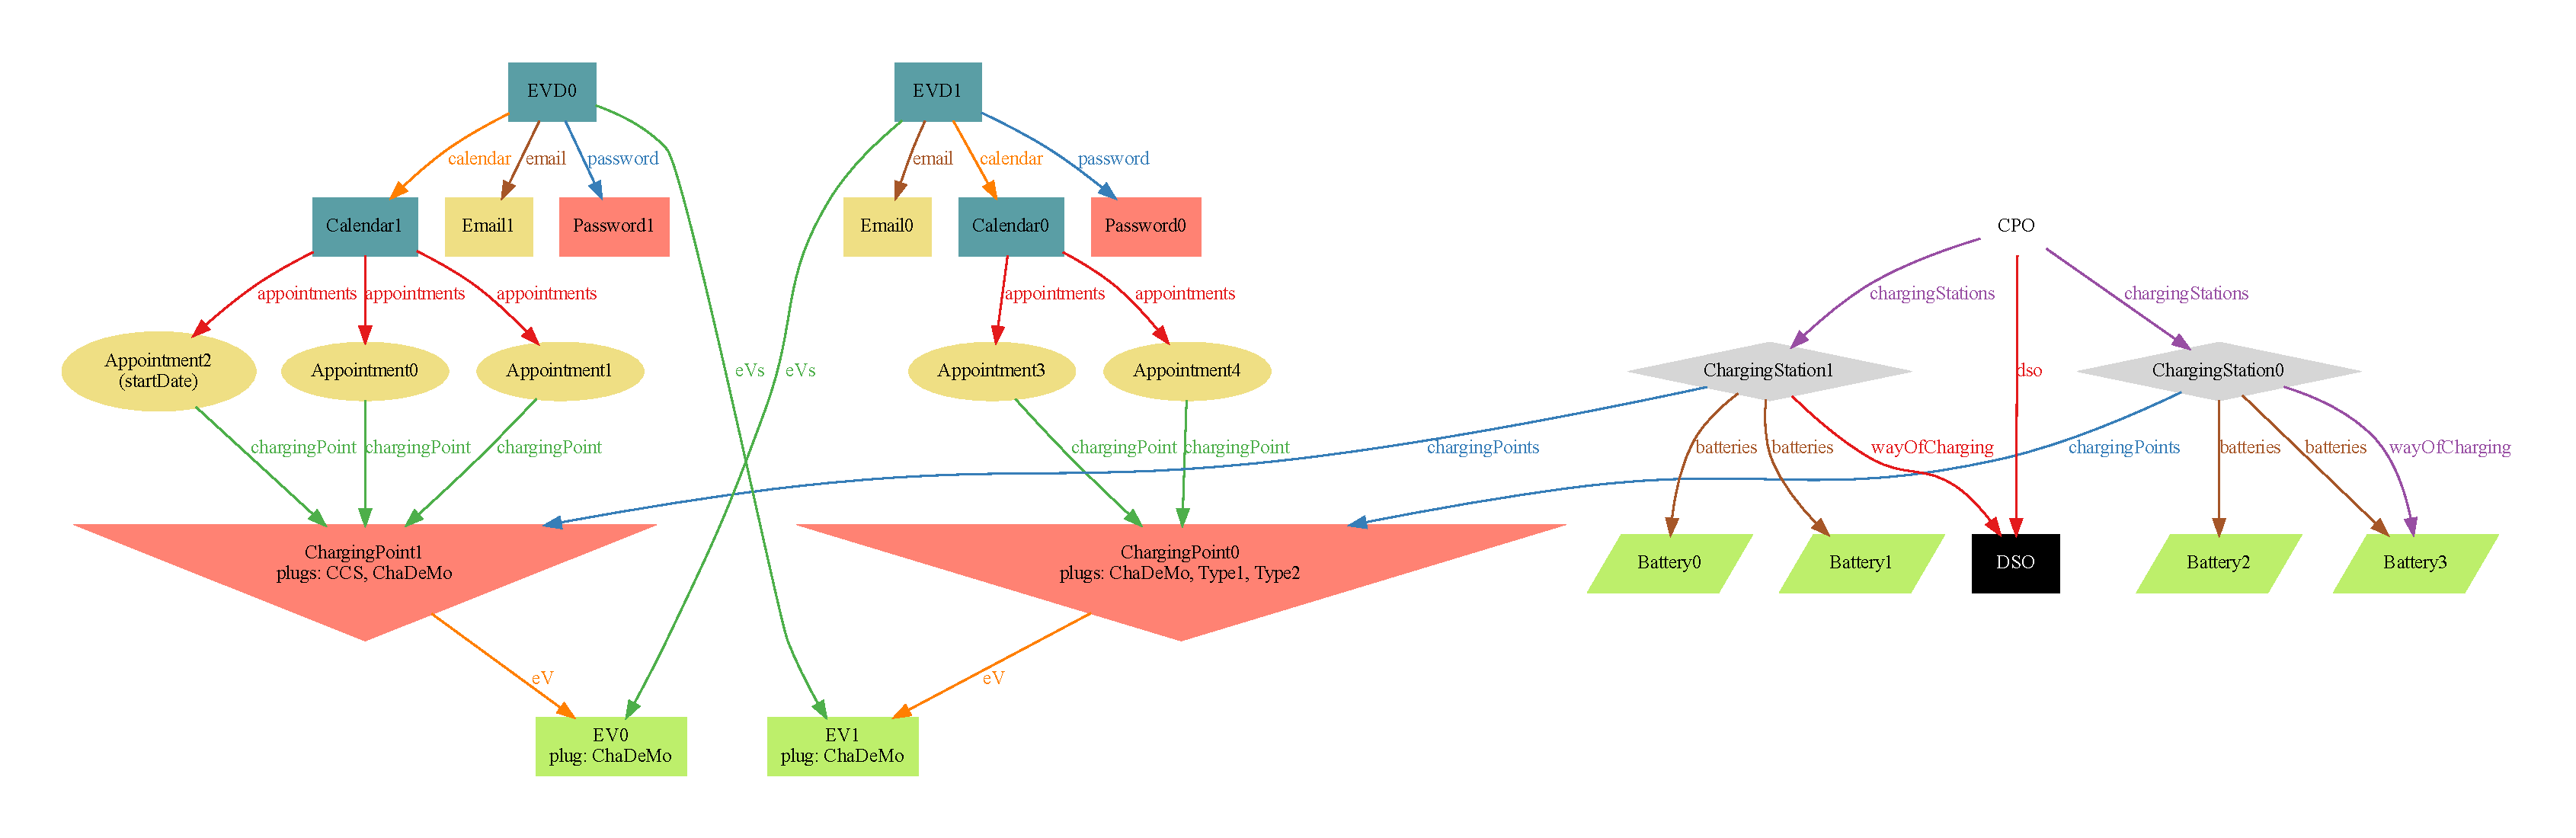
\includegraphics[width=1\linewidth]{graphs/worldWithManyAppointments}
			\caption{More complex world.}
			\label{fig: many_appointments_world_alloy}
		\end{center}
	\end{figure}
\end{sidewaysfigure}
